\documentclass[12pt,a4paper]{article}
\newcommand{\AuthorName}
{حسن ذاکر، علیرضا دقیق، سپهر فعلی}
\newcommand{\AuthorSTID}
{96105778,96105723,96105959}

\usepackage{float}


\usepackage{listings}
\usepackage{courier}
\lstset{
tabsize = 4, %% set tab space width
showstringspaces = false, %% prevent space marking in strings, string is defined as the text that is generally printed directly to the console
numbers = left, %% display line numbers on the left
commentstyle = \color{green}, %% set comment color
keywordstyle = \color{blue}, %% set keyword color
stringstyle = \color{red}, %% set string color
rulecolor = \color{black}, %% set frame color to avoid being affected by text color
basicstyle = \small \ttfamily , %% set listing font and size
breaklines = true, %% enable line breaking
numberstyle = \tiny,
}
\lstloadlanguages{ % Check documentation for further languages ...
     % [Visual]Basic,
     % Pascal,
     % C,
     % C++,
     % XML,
     % HTML,
     Java
}
% \DeclareCaptionFont{blue}{\color{blue}} 

% \captionsetup[lstlisting]{singlelinecheck=false, labelfont={blue}, textfont={blue}}
\usepackage{caption}
\DeclareCaptionFont{white}{\color{white}}
\DeclareCaptionFormat{listing}{\colorbox[cmyk]{0.43, 0.35, 0.35,0.01}{\parbox{\textwidth}{\hspace{15pt}#1#2#3}}}
\captionsetup[lstlisting]{format=listing,labelfont=white,textfont=white, singlelinecheck=false, margin=0pt, font={bf,footnotesize}}


\usepackage{commons/course}




% ما ۳ نفر همه سوالات را با هم حل کردیم.

%
%\let\ds\displaystyle
%\usepackage{arabtex}
%\usepackage[utf8]{inputenc}
%\usepackage[LFE,LAE]{fontenc}
%\usepackage[english,farsi]{babel}
%


\begin{document}



\سربرگ{پاسخ تمرین سری سوم}{\lr{SDT, Scope, Type Checking}}{99/09/22}


\textbf{ما ۳ نفر همه سوالات را با هم حل کردیم}
\newline
%نام و نام خانوادگی:
%شماره دانشجویی: 
\مسئله{طراحی \lr{DFA}}

\پاسخ{}



%نام و نام خانوادگی:
%شماره دانشجویی: 
\مسئله{عبارت آرمانی}

\پاسخ{
\begin{enumerate}
	\item
	علاوه بر پارس‌استک PS 
	یک استک جدید به نام TS تعریف می‌کنیم که در هنگام پارس کردن به کمک ما می‌آید. به این صورت که هر موقع + داشتیم آن را به TS اضافه می‌کنیم و هرگاه یه - رسیدیم از استک TS POP می‌کنیم.
	 عملیات پارس به‌صورت معمول با PS انجام می‌شود و علاوه بر حالت‌های invalid که ممکن است در PS رخ دهد زمانی که باید از TS POP کنیم و TS خالی باشد نیز باید حالت invalid تشخیص داده‌شود.
		\begin{figure}[H]
			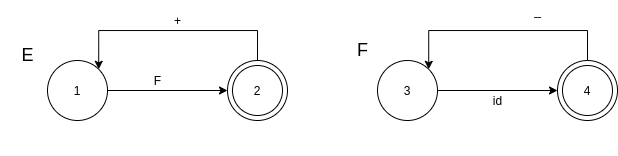
\includegraphics[width=\linewidth]{./commons/Q2part1.png}
			\label{fig:Q2}
		\end{figure}
	\item
	از آنجایی که بعد از دیدن - حتما یک‌بار باید F را ببینیم و اگر id دیگری بخواهد بیاید حتما باید T را ببینیم و در ابتدای T حتما + می‌بینیم، حالت‌های valid پارس خواهند شد و حالت‌های invalid قابل پارس شدن با استفاده از PS نیستند.
		\begin{figure}[H]
			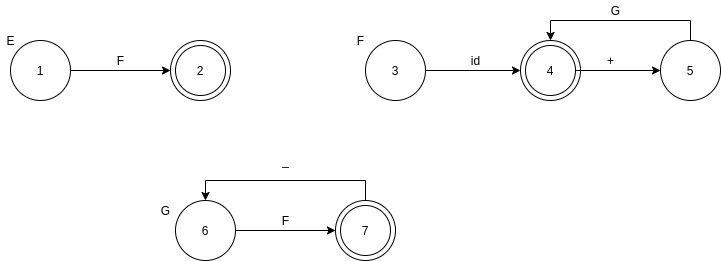
\includegraphics[width=\linewidth]{./commons/Q2part2.png}
			\label{fig:Q2}
		\end{figure}
\end{enumerate}
}


%نام و نام خانوادگی:
%شماره دانشجویی: 
\مسئله{\lr{Syntax Graph}}

\پاسخ{
\newline
اصلاح گراف:
\newline
\begin{itemize}
	\item {
روال مفهومی \lr{@push} را روی یال \lr{s8} به \lr{s9} قرار میدهیم. (\lr{id/@push})
	}
	\item{
روال مفهومی \lr{@add} را روی یال \lr{s3} به \lr{s2} قرار میدهیم. (\lr{T/@add})
	}
	\item{
روال مفهومی \lr{@mult} را روی یال \lr{s7} به \lr{s6} قرار میدهیم. (\lr{F/@mult})
	}
\end{itemize}


گرامر:
\newline
\begin{latin}

	\begin{itemize}
		\item E $\rightarrow$ TE'
		\item E' $\rightarrow$ +TE'
		\item E' $\rightarrow$ $\lambda$
		\item T $\rightarrow$ FT'
		\item T' $\rightarrow$ *FT'
		\item T $\rightarrow$ $\lambda$
		\item F $\rightarrow$ id
		\item F $\rightarrow$ (E)
	\end{itemize}

	\begin{table}[H]
		\begin{tabular}{c|c|c|c}
			token & remain & PS & SS\\
			\hline
			 & id + id & \$ &  \\
			 id & + id & E \$ &  \\
			 id & + id & T E' \$ &  \\
			 id & + id & F T' E' \$ &  \\
			 id & + id & \&push id T' E' \$ &  \\
			 id & + id & id T' E' \$ &  \\
			 + & id & T' E' \$ & id \\
			 + & id & E' \$ & id \\
			 + & id & + T \&add E' \$ & id \\
			 id &  & T \&add E' \$ & id \\
			 id &  & F T' \&add E' \$ & id \\
			 id &  & \&Push id T' \&add E' \$ & id \\
			 id &  & id T' \&add E' \$ & id \\
			  &  & T' \&add E' \$ & id id \\
			  &  & \&add E' \$ & id id \\
			  &  & E' \$ & t \\
			  &  & \$ & t\\

		\end{tabular}
	\end{table}
\end{latin}

}



%نام و نام خانوادگی:
%شماره دانشجویی: 
\مسئله{تبدیل \lr{NFA}  به \lr{DFA} }

\پاسخ{}

%نام و نام خانوادگی:
%شماره دانشجویی: 
\مسئله{}
\پاسخ{}
   
\end{document}

